% Chapter 3

\chapter{Discussion and Results Obtained} % Main chapter title

\label{Chapter4} % For referencing the chapter elsewhere, use \ref{Chapter4} 

%----------------------------------------------------------------------------------------

\section{Discussion and Results Obtained}

\subsection{Discussions}

\subsubsection{Hours spent at work everyday}

During my internship period, I make sure i report to work at 9am and leave at 5pm making a total of 8 hours per day. Working days are from Monday to Friday and during the weekends, we are officially not allowed to work but if there is something someone wants to work on in the office during the weekend, he/she seeks permission from the Owner of the company in order to notify the attention of the company.

\subsubsection{How was work carried out each day?}

Before we start working each day, task are assigned to us either by the project lead or the overall founder of the project and we make sure to finish the task given to us by the end of the week and if its difficult and require some research, we shall use 2 - 3 weeks to finish the task and there are some minor task that take a few hour to finish but some take days. \\

Depending on the work load, before departing from the office to the house, the work I have done that day and including all the other interns are shown to the owner of the project or the project lead to review it and if there is any corrections that can be done quickly, we fix it but if it can't be done immediately, we carry it over to the next day. \\

\subsubsection{Submission of task to be Intergrated to the main project}

At the end of each task, when I see that its possible to integrate my work into the main software online, I push my codes to my repository online and send a pull request to the project leave to do a final review before merging the codes to the main repository. This means every intern working on nukeboard had a separate  repository of the project online but there was a main one that was only used to merge only working codes so that we won't be mess up the main repository. Below is the contributors page for all users contributing to the nukeboard project;

\begin{figure}[h]
\centering
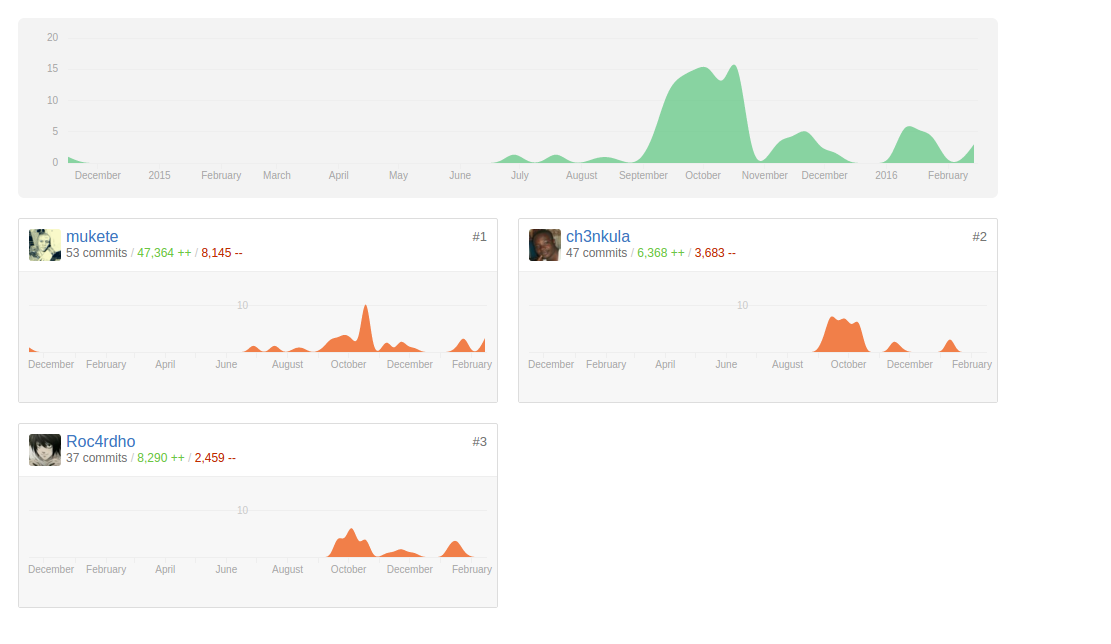
\includegraphics[width=13cm,scale=1.5]{Figures/GitHubProject}
\decoRule
\caption[Nukeboard Code Contributors]{Contributors of codes to Nukeboard}
\label{fig:GitHubProject}
\end{figure}

\subsubsection{General discussion about entire work done}

   Generally, the work I did for 5 months during my internship was a great contribution to the success of this project. Together with my other colleagues, we made sure that when doing a task, we should work on the task very well such that the software in general will be almost perfect and if there is any change we are not make, it will not cost us rebuilding the whole software from scratch. \\
   
In addition to this, we as the nukeboard team worked very much in collaboration both online and offline to make sure that the project goes well and task are accomplished on time and accurately. Also we code in such a way that if a task is given to us and another colleague has to complete it when we are not available, he/she is not stressed up in order to understand the code since its well commented and documented for ease of understanding.

\subsection{Results Obtained}

At this point, results obtained after carrying out all my tasks during my internship period will be revealed. In addition to the above mentioned outcomes(results) where snap-shots where inserted and textual results mentioned, I will also reveal more results here concerning the outcomes as regards my work done during internship.

\subsubsection{Quality Assurance for Nukeboard}

\begin{tabular}{ |p{3cm}|p{3cm}|p{3cm}|  }
 \hline
 \multicolumn{3}{|c|}{Quality Assurance Statistics} \\
 \hline
 Test Cases & \% passed & \% failed \\
 \hline
 53  & 75.47\% & 24.53\% \\
 \hline
\end{tabular}

Testing of the whole software took me 1 month and at the end of the month, I did not still finish testing the whole software but the statistics in the table above reveals the performance and out come of the system including my work and the work of other interns concerning the project. 